\documentclass[twocolumn,numberedappendix]{../aastex6}

% these lines seem necessary for pdflatex to get the paper size right
\pdfpagewidth 8.5in
\pdfpageheight 11.0in

% for the red MarginPars
\usepackage{color}

% some extra math symbols
\usepackage{mathtools}

% allows Greek symbols to be bold
\usepackage{bm}

% allows us to force the location of a figure
\usepackage{float}

% allows comment sections
\usepackage{verbatim}

% Override choices in \autoref
\def\sectionautorefname{Section}
\def\subsectionautorefname{Section}
\def\subsubsectionautorefname{Section}

% MarginPars
\setlength{\marginparwidth}{0.75in}
\newcommand{\MarginPar}[1]{\marginpar{\vskip-\baselineskip\raggedright\tiny\sffamily\hrule\smallskip{\color{red}#1}\par\smallskip\hrule}}

\newcommand{\msolar}{\mathrm{M}_\odot}

% Software names
\newcommand{\amrex}{\texttt{AMReX}}
\newcommand{\boxlib}{\texttt{BoxLib}}
\newcommand{\castro}{\texttt{CASTRO}}
\newcommand{\microphysics}{\texttt{Microphysics}}
\newcommand{\wdmerger}{\texttt{wdmerger}}
\newcommand{\python}{\texttt{Python}}
\newcommand{\matplotlib}{\texttt{matplotlib}}
\newcommand{\yt}{\texttt{yt}}
\newcommand{\vode}{\texttt{VODE}}
\newcommand{\isoseven}{\texttt{iso7}}
\newcommand{\aproxthirteen}{\texttt{aprox13}}
\newcommand{\aproxnineteen}{\texttt{aprox19}}
\newcommand{\aproxtwentyone}{\texttt{aprox21}}

\begin{document}

%==========================================================================
% Title
%==========================================================================
\title{White Dwarf Mergers on Adaptive Meshes\\ II. Nuclear Reactions}

\shorttitle{WD Mergers. II. Nuclear Reactions}
\shortauthors{Katz et al. (2017)}

\author{Max P. Katz\altaffilmark{1}}
\author{Michael Zingale\altaffilmark{1}}
\author{Alan C. Calder\altaffilmark{1,2}}
\author{F. Douglas Swesty\altaffilmark{1}}
\author{Ann S. Almgren\altaffilmark{3}}
\author{Weiqun Zhang\altaffilmark{3}}
\author{Frank X. Timmes\altaffilmark{4,5}}

\altaffiltext{1}
{
  Department of Physics and Astronomy,
  Stony Brook University, Stony Brook, NY, 11794-3800, USA
}

\altaffiltext{2}
{
  Institute for Advanced Computational Sciences,
  Stony Brook University, Stony Brook, NY, 11794-5250, USA
}

\altaffiltext{3}
{
  Center for Computational Sciences and Engineering,
  Lawrence Berkeley National Laboratory, Berkeley, CA 94720
}

\altaffiltext{4}
{
  The Joint Institute for Nuclear Astrophysics, USA
}

\altaffiltext{5}
{
  School of Earth and Space Exploration, Arizona State University, Tempe, AZ, USA
}



%==========================================================================
% Abstract
%==========================================================================
\begin{abstract}
Simulations of white dwarf mergers and collisions that attempt to answer the
question of whether these events are progenitors of Type Ia supernovae must
confront the question of how nuclear detonations form and whether observed
detonations in a numerical simulation are realistic. We address this question
by performing simulations of collisions of white dwarfs, a subset of white
dwarf mergers that occur when the stars approach each other nearly head-on.
These have the potential for explosive nucleosynthesis, leading to a thermonuclear
detonation that disrupts both stars, possibly causing a Type Ia supernova.
While this story is intuitively plausible, demonstrating this in a reacting
hydrodynamics simulation is challenging due to the rapid evolution of the
nuclear burning, posing numerical challenges related to both spatial and
temporal resolution. In this study we explore a number of the algorithms
that affect the outcome of reacting hydrodynamics simulations that lead
to explosive burning and address the question of what can be done to ensure
that these simulations are properly converged. We find that achieving a
converged simulation in the code \castro\ is very difficult for a standard
approach with uniform resolution. The typical timesteps taken by hydrodynamics
codes are too large and the spatial resolution is too low, while increasing
either to the point required to actually obtain a converged simulation is
prohibitive. However, we have identified a criterion for adaptive mesh refinement
that substantially improves the situation: by targeting for extra sptial resolution
only those regions that are likely to undergo numerically unstable burning,
we can significantly reduce the effects of numerically spurious detonations.
This result is a possible path forward for obtaining reliable numerical
simulations of Type Ia supernova involving thermonuclear detonations.
\end{abstract}
\keywords{supernovae: general - white dwarfs}

%==========================================================================
% Introduction
%==========================================================================
\section{Introduction}
\label{sec:introduction}

Binary white dwarf (WD) systems are a promising progenitor candidate for Type
Ia supernovae (SNe Ia) for observational reasons, but from the simulation
perspective there is still significant uncertainty regarding how nuclear
detonations form in an exploding white dwarf. There is uncertainty in the
model, regarding whether detonations form on the surface of a star as
accreting material heats up when it strikes the surface, or at or near the
center of the star as the accreted material compresses the WD. There is also
uncertainty in the numerics: given one of these models, can we self-consistently
demonstrate that a detonation occurs? This question has haunted both single
WD and double WD progenitor models, because the length and time scale at which
a detonation forms is orders of magnitude smaller than the resolution that
typical hydrodynamic simulations can achieve. Furthemore, the approximate equations
we use at the resolution that we can achieve are still notoriously
difficult to solve accurately. The mere presence of a detonation
(or lack thereof) in a simulation is therefore only weak evidence regarding
whether a detonation would truly occur.

In this study we examine the challenges associated with simulating nuclear detonations.
This paper follows from our first WD merger methodology paper, \citet{wdmergerI}
(hereafter, Paper I), where we deferred discussion of our nuclear reaction methodology.
After presenting the burning methodology, we apply it to the problem of collisions of white dwarfs.
WD collisions can occur in isolated binaries or in hierarchical triple systems, where the WD binary
system in a tight inner orbit is gravitationally coupled to a third, outer star \citep{thompson:2011,hamers:2013}.
Whether the rate of these collisions may be high enough to significantly contribute to
the observed SN Ia rate is debated: \cite{katzdong:2012} suggest that this is plausible,
but \cite{hamers:2013} and \cite{papish:2015} suggest that the rate is relatively low.
Regardless, they are a useful vehicle for understanding the problem of nuclear burning.
Head-on WD collisions rapidly convert a significant amount of kinetic energy into thermal
energy in a small region and thus set up conditions ripe for a thermonuclear detonation;
being able to correctly simulate these is in some sense a prerequisite to correct simulation
of the more complicated general case of white dwarf mergers, where we do not initially know
under what conditions the seed of a thermonuclear detonation is born.

There have been a number of previous studies which provide useful insight into setting up
the problem and the burning methodology \citep{rosswog:2009,raskin:2010,loren-aguilar:2010,
hawley:2012,garcia-senz:2013,kushnir:2013,papish:2015,holcomb:2015}. These studies
found that detonations occur and convert a large amount of carbon/oxygen material into
iron-group elements. These papers varied significantly in the hydrodynamic methods used
(Lagrangian versus Eulerian methods), the methodology used for coupling nuclear
reactions to the hydrodynamics (including variation in the number of isotopes in
the nuclear network and in the evolution of the temperature), and the temporal and
spatial resolution. Consequently the detonations they formed varied in location and nature,
and the resultant estimates of production of nickel-group elements varied significantly,
leaving much uncertainty about how such an event would appear observationally and whether
it bears any resemblance to a SN Ia. See Table 4 of \cite{garcia-senz:2013} for a summary
of the outcome of many of these studies. In this paper we make the case that
while we can identify the main problems prevent accurate simulation of the collision
event, there is no clear path to overcoming them using the computational resources
typically available for contemporary hydrodynamics simulations.

%==========================================================================
% Numerical Implementation
%==========================================================================
\section{Numerical Methods}
\label{sec:numericalmethods}

The hydrodynamical equations solved in this paper were presented in \citet{wdmergerI}
(hereafter, Paper I) for the reacting hydrodynamics code \castro\ \citep{castro}.
Only minor revisions to the core hydrodynamic algorithm have since occurred.
In this paper we focus our discussion on our implementation of the nuclear
reaction network and integrator. There are three main areas of concern: first,
specifying what nuclides are in the network and what reaction rates link the
various nuclides; second, once the system of ODEs governing the evolution of
the nuclear species has been written down, how to couple them to ODEs governing
the evolution of the thermodynamics, in particular the temperature; third,
coupling the nuclear reaction updates to the evolution of the hydrodynamical
system. We will deal with each of these in turn in the following subsections.

\subsection{Nuclear Network}
\label{sec:network}

White dwarfs are mainly composed of $\alpha$-chain particles, primarily ${}^4$He,
${}^{12}$C, ${}^{16}$O, ${}^{20}$Ne, and ${}^{24}$ Mg. Therefore the core of
any network appropriate for modeling nuclear burning in white dwarfs will be
these alpha chain nuclides, with the idea being that links up the $\alpha$-chain
will eventually get us to ${}^{56}$Ni, the nuclide responsible for the
energy output of Type Ia supernovae. In this paper we use the \aproxthirteen\
network\ \citep{timmes:1999,timmes:2000}. This includes all thirteen $\alpha$-chain
particles between ${}^4$He and ${}^{56}$Ni. This network was used by \citet{hawley:2012}
and \citet{raskin:2010}. \citet{loren-aguilar:2010} and \citet{garcia-senz:2013} used a
very similar network that additionally included ${}^{60}$Zn. This network has been
ported into a form that is consistent with the \amrex\ codes, in the freely available
\microphysics\ code repository
\footnote{\microphysics\ can be obtained at \url{https://github.com/starkiller-astro/Microphysics}.},
a collection of microphysical routines that are designed to be used in our
hydrodynamics codes. In our \microphysics\ repository we have also ported \aproxnineteen\
\citep{timmes:1999}, which was used in a few previous collision papers, and \aproxtwentyone.
The isotopes added by these networks relative to \aproxthirteen\ are not particularly relevant
to the problem of head-on white dwarf collisions, so we do not discuss results with these networks
here (though we have verified for this problem that these larger networks do not significantly change
the answer). We also make available \isoseven\ \citep{timmes:2000}, which skips the nuclides between
silicon and nickel, and was used by \citet{rosswog:2009}. \isoseven\ gives significantly different
quantitative results than \aproxthirteen\ for this problem, due to the inapplicable assumption of
an equilibrium abundance of the unused isotopes, but the results are still qualitatively similar.

\subsection{Nuclear Burning}
\label{sec:burner}

Given a set of nuclides and the reaction links between them, we now consider
how a burning step is performed in our software. The goal is to integrate the
vector ${\bm{Y}} = (Y_1, Y_2, \ldots, Y_n, e, T)$, where $Y_{n} = X_{n} / A_{n}$
is the molar fraction of species $n$, with $X_n$ the mass fraction and $A_n$ the
mass number of that species, $e$ is the energy released during the burn, and
$T$ is the temperature. The equation describing its evolution is given by
\begin{equation}
  \frac{d\bm{Y}}{dt} = f(\mathbf{Y}),
\end{equation}
where the components of the right-hand-side for the species come from the particular
nuclear burning network we are using. The energy $e$ of the zone
will change when the nuclear abundances evolve, according to
\begin{equation}
  \frac{\partial e}{\partial t} = N_A \sum_{n} \frac{\partial Y_{n}}{\partial t} m_{n} c^2,
\end{equation}
where $c$ is the speed of light and $m_n$ is the mass of each nuclide.

We define several burning modes that determine how $T$ and $e$ are evolved
during a nuclear burn. In a hydrostatic burn, which we call burning mode 0,
we keep $\rho$ and $T$ fixed throughout, and use 
the energy released at the end to compute a final temperature that is
thermodynamically consistent with the new internal energy. By contrast,
in a self-heating burn (mode 1), we allow the temperature to evolve in response
to the burning (see\footnote{In the cited paper, a term based on the
thermodynamic chemical potential was included; we now believe
that it is incorrect to include such a term in the burn, since it
automatically sums to zero analytically.} \citet{maestro3}):
\begin{equation}
  \frac{dT}{dt} = \frac{1}{c_V}\frac{\partial e}{\partial t}
\end{equation}
(Although $T$ evolves during the burn so that the integration is physically
accurate, as in the hydrostatic method we discard the final value
for $T$ at the end of the burn and recompute a temperature for the zone that is
consistent with its new internal energy.) Here $c_V$ is the specific heat at
constant volume, which is provided by the equation of state.  During this burn,
we can keep $c_V$ constant using its initial value, or at each step we
can choose to re-evaluate the equation of state using the latest value of $(\rho, T)$.
The latter is more expensive but also more accurate, and we use it in this paper.
In practice we find that the cost is small in comparison to the more expensive
parts of the calculation, and it can significantly speed up convergence near NSE.
A third option (mode 2) presented by \citet{raskin:2010} is a so-called ``hybrid'' mode.
In this mode, by default we do a hydrostatic burn. If that burn fails, or if the net
energy change is negative, we do the burn again in self-heating mode. A final option (mode 3)
is a burn that limits the changes due to a burn to avoid numerically unstable burning.
This mode is discussed in \autoref{sec:unstable_burning} and we will call it a
``suppressed'' burn for the remainder of this work. All four options
are implemented in our burner software. The simulations shown in this work all
use the self-heating mode unless otherwise specified.

In our \microphysics\ repository we provide several software options for
solving a set of coupled stiff ODEs. For this work our primary integrator
is the classic \vode\ integrator \citep{vode}, of which we have a version
compatible with our software interfaces in the \microphysics\ repository.
We also employ an implementation of the well known variable-order Richardson
extrapolation method presented by \citet{stoer:1980}, that is similar to the
integrator which ships with the original versions of the networks mentioned
above. Our experience shows that relying on a single ODE integrator for the
variety of stiff ODEs that are present in a collision is insufficient, as we
sometimes run into integration failures. A combination of the two integrators
is usually sufficient, however: we first try \vode, and if that fails, we then
try the Stoer and Bulirsch method. Since it is possible for neither method to
succeed, we have one more backup scheme. Our specified (relative and absolute)
error tolerances are uniformly $10^{-6}$ for the energy, temperature, and nuclear
abundance ODEs. We can loosen these tolerances in an attempt to give the integrator
an easier time. If both \vode\ and the Stoer and Bulirsch algorithm fail, then we
loosen the tolerances by a multiplicative factor of 25\%, and then repeat the attempts
with \vode\ and Stoer and Bulirsch. We keep doing this until either we have loosened
the tolerances enough for one of the two methods to succeed, or until we have loosened
the tolerances by two orders of magnitude, at which point we finally give up. We have
found that this scheme is resilient enough to handle all of the simulations shown below.
We have also verified that our results do not depend much on the tolerances when they
are tighter than $10^{-4}$.

\subsection{Coupling to the Hydrodynamics}
\label{sec:hydrocoupling}

In \castro, the reactions are coupled to the hydrodynamics using Strang splitting.
In a given timestep advance $\Delta t$, we first evolve the reactions alone through
a time interval $\Delta t / 2$. Then, we evolve the hydrodynamics for $\Delta t$,
and we evolve the reactions again for a further $\Delta t / 2$. The principal
drawback of this approach is that the reactions and the hydrodynamics can become
decoupled from each other. A common solution to this problem presented in
the literature has been to limit the size of the timestep and thereby limit the
extent of this decoupling \citep{raskin:2010,hawley:2012}, which we adopt here 
and have implemented in \castro. Defining the nuclear energy injection timescale 
$\tau_e$, and the species evolution timescale $\tau_{X_k}$,
\begin{align}
  \tau_e &\equiv \frac{e}{|\dot{e}|} \\
  \tau_{X_k} &\equiv \frac{X_k}{|\dot{X_k}|},
\end{align}
where $\dot{e}$ is an estimate of the time rate of change of the internal energy
from nuclear burning, and $\dot{X_k}$ is an estimate of the time rate of change 
of the mass fraction of the species with index $k$, we define burning-limited 
timesteps $\Delta t_{be}$ and $\Delta t_{bX_k}$:
\begin{align}
  \Delta t_{be} &= f_{e}\, \tau_e \label{eq:timestep_e}\\
  \Delta t_{bX_k} &= f_{X}\, \tau_{X_k}. \label{eq:timestep_X}
\end{align}
Given an estimate for $\dot{e}$, the factor $f_{e}$ determines by what 
fraction we would like to allow the internal energy to change
in the current timestep, under the assumption that $\dot{e}$ does not change from
timestep to timestep. Similarly, given an estimate for $\dot{X_k}$, the factor $f_{X}$ 
determines the maximum change in the mass fraction of any species. To prevent species
whose abundances are small in absolute terms from controlling the timestep, we apply
the limiter based on $f_{X}$ only to species with abundances in a given zone greater
than $10^{-3}$ (this abundance threshold can be changed by the user of the code). By making 
$f_{e}$ and $f_{X}$ smaller, we can control the magnitude of the decoupling 
between the reactions and the hydro. A typical choice for $f_e$ parameter in the
literature is in the range of 0.2 or 0.3, while to our knowledge a limiter based on
$f_X$ has not been used by others performing these types of calculations. The sensitivity
of results to the value of these timestep limiters will be discussed in 
\autoref{sec:parameters:timestepping}. The factors $f_{e}$ and $f_{X}$ can be set at runtime in \castro.

At the start of each advance, we limit the size of the timestep to be the smaller
of the minimum hydro timestep (limited by the CFL condition), and the minimum of all the
burning timesteps across all zones. To do this, we need a method for determining 
$\dot{e}$ and $\dot{X_k}$. A typical choice in the literature has been to set, for example,
\begin{equation}
  \dot{e} = \frac{e^{n} - e^{n-1}}{\Delta t^{n-1}}, \label{eq:burning_limiter_mode_4}
\end{equation}
where is $e^n$ is the internal energy at the start of the current timestep and
$e^{n-1}$ is the internal energy at the start of the previous timestep. 
The obvious analogue is used for constructing the species rate of change.
However, there are alternative methods of constructing this derivative estimate, 
and we have found that these different methods have measurable consequences.
We define four separate methods for calculating the time derivative, with 
the above being mode 4. Mode 3 is similar to mode 4 but replaces the
denominator in \autoref{eq:burning_limiter_mode_4} with the change in 
internal energy over the last timestep only from the nuclear reactions.
Mode 2 is the same as mode 3 but we only use the change in internal 
energy from the most recent nuclear burning step, that is, the second-half
of the Strang-split burning from the last timestep (the denominator 
then becomes $\Delta t / 2$). In mode 1, the most accurate option and 
the current default in \castro, we evaluate the right-hand-side of the 
burning network given the current state to explicitly obtain the 
instantaneous value of $\dot{e}$ and $\dot{X_k}$. 

%TODO: add a ``Nonaka plot''

To understand the consequences of this choice, and more broadly to 
understand the limitations of Strang splitting, we consider the 
basic outline of a single-level advance in an advection-reaction system:
\begin{enumerate}
  \item Evaluate timestep $\Delta t$ for the current advance
  \item Advance the nuclear burning network by $\Delta t / 2$
  \item Advance the hydrodynamics by $\Delta t$
  \item Advance the nuclear burning network by $\Delta t / 2$
  \item Return to Step 1
\end{enumerate}
Now, consider that during a head-on collision, initial nuclear burning 
will occur at the contact point between the two stars. Because of 
the staggered updates from splitting, the evolution effectively progresses 
as a cycle between burning for $\Delta t$ and getting fresh material 
advected into the contact point by the hydro update for $\Delta t$. 
When the collision begins, $\Delta t$ is controlled by the hydrodynamic 
stability criterion, and may be large enough that it is possible for 
the burning advance in Step 4 to completely burn the freshly advected 
material all the way to NSE. Consequently the evolution is no longer 
a good approximation to smooth burning of the in-falling material but
rather separate discrete burning and hydro steps, and the nature of 
the burning evolution will be quite different. Furthermore, by the 
time we return to Step 1 and estimate the next timestep size, all 
of the burning rates will be small again, and the instantaneous 
timestep limiter of mode 1 may actually substantially overestimate 
the needed timestep. The other modes will see that the energy/species  
substantially changed over the last timestep, but will still
overestimate the needed timestep because the burning was quiescent
for at least some portion of the last advance. Our experience has
shown that none of these methods is flawless, and that limiting
based on only changes in internal energy is particularly susceptible
to this staggered burning phenomenon; silicon-group material can
build up without changing the internal energy by a  large fraction,
so the timestep limiter is never triggered, and then in a single step
a substantial amount of iron-group elements can be be generated,
perhaps forming a detonation. In practice, however, we find that
this effect is not large enough to have a meaningful outcome, and
the results are largely insensitive to which method of limiting
is used.

With the timestep limited the way we advocate in this paper, 
the timesteps are generally short enough so that the errors 
due to splitting are small. Other approaches to the coupling 
between reactions and hydrodynamics have been proposed in the 
broader literature, especially iterative methods such as 
deferred corrections that allow each of these operators to 
feel the lagged effects of the other operators. For example,
in the context of low Mach number flows, \cite{nonaka:2012} have
used the method of spectral deferred corrections \citep{SDC} to
couple their advection-diffusion-reaction equation set. In our
context this would involve treating the full evolution equation
for each of the state variables as an ODE with a directly coupled
burning source term integrated at high order; the advective
flux is evaluated at the standard second order accuracy
and is included as an ODE source term.
We are presently investigating such a method,
and it may form the basis of further work on this subject.

Now we return to a point we hinted at above. The timestep
will only actually satisfy the energy criterion
$\Delta t \leq f_e \tau_e$ and species criterion
$\Delta t \leq f_{X_k} \tau_{X_k}$ when the estimates for
$\dot{e}$ and $\dot{X_k}$ we generate are at least as large
as the actual rate of change of energy and mass fractions
over the timestep. However, this can assumption can fail
during periods of runaway burning when the rate of change
of these quantities is highly nonlinear. We may not want
to neglect the errors caused by this approximation
because they may build up over an extended period of nonlinear
evolution and perhaps substantially change the final results.
To this end, we have implemented a timestep retry option in
\castro, which re-computes an advance if it violated the
stability criteria as judged from the end of the timestep.
We have found that the benefits for this problem are, however, small.

\subsection{Numerically Unstable Burning}
\label{sec:unstable_burning}

\citet{kushnir:2013} point out that an inappropriate timestep is 
not the only way for the numerical discretization to cause 
severe errors in the burning. Another failure mode is when
the energy injection timescale
$\tau_e$ is shorter than the sound-crossing time $\tau_s$ in a zone.
When the sound-crossing time is too long, energy is built up in
a zone faster than it can be advected away by pressure waves.
This is obviously a problem inherent to numerically discretized
systems as the underlying fluid equations are continuous.
This can lead to a numerically seeded detonation caused by the
temperature building up too quickly in the zone; the detonation
is spurious in this case and should be avoided if possible.
The goal is to ensure that the following condition holds:
\begin{equation}
  \tau_s \leq f_{s}\, \tau_e \label{eq:burning_limiter_2}
\end{equation}
The sound crossing time, $\tau_s$, is given by $\Delta x / c_s$, 
where $c_s$ is the sound speed and $\Delta x$ is the (minimum) 
zone width. The parameter $f_{s}$ then determines the minimum
ratio of the nuclear energy generation timescale to the 
sound-crossing time. \citet{kushnir:2013} choose $f_{s} = 0.1$ 
for their simulations, and we do too (this parameter can be set 
at runtime in \castro).

\citet{kushnir:2013} implemented this criterion by artificially 
limiting the magnitude of the energy release after a burn. We
too have developed an option for our burner to do this,
the ``suppressed'' burning mode. In a suppressed burn, we limit
the changes to the state so that \autoref{eq:burning_limiter_2}
is always satisfied. To achieve this we directly multiply the
right-hand-side vector in the integration by a constant factor $F$
for all variables, where $F$ is the multiplicative factor needed to
be applied to $\dot{e}$ such that the equality in \autoref{eq:burning_limiter_2}
holds. (If the inequality is already satisfied, then the integration
vector is not modified.) We fix $\tau_s$ to be the value of the sound
crossing time at the beginning of the burn (that is, we do not
update it as the sound speed changes) and we fix the energy $e$
that goes into the estimate for $\tau_e$ to be the value of the
internal energy of the zone at the beginning of the burn. If
instead one allowed $c_s$ and $e$ to evolve with the burn, one
would obtain a less conservative limiter in the case of explosive
burning, as $c_s$ and $e$ are both increasing in this case.
As the point of the limiter is to ensure that the changes to the
\textit{original} energy are small enough so that the following
hydrodynamics update can advect away newly generated energy
quickly enough to avoid a numerically seeded detonation,
we desire the most conservative version of the limiter. We discuss
our results with the suppressed burning mode in \autoref{sec:collisionburning}.
Note that we have found that with this option enabled, it typically takes
many more timesteps to complete a burn than in self-heating mode.

Regardless of whether the suppressed burning mode works for this
particular problem, it is not physical, so we include for
consideration a different approach. If we insist that we
cannot directly control the energy injection timescale, we 
must find a way to alter the sound-crossing timescale. 
We can achieve this by adding levels of refinement in 
regions that do not satisfy \autoref{eq:burning_limiter_2},
which effectively lowers $\Delta x$ and thus the
sound-crossing time. We keep tagging zones for refinement
based on this criterion until the criterion is satisfied
on the finest level. Since the concern is regions that 
may detonate, we also tag nearby zones in a buffer region
which do not themselves satisfy the criterion,
so that a detonation in a single timestep cannot 
escape into non-refined regions. The width of the buffer 
region should thus be at least as large as the number of 
timesteps before a regridding procedure is performed.
We choose a value of two for both the number of zones in the 
buffer region and the number of steps in between regrids,
for all simulations in this paper.

We agree with \citet{kushnir:2013} that solving this numerical
instability is crucial to avoiding unphysical detonations.
A simulation that does not solve this problem will not obtain
the correct amount and will not converge properly with resolution.
This may justify the addition of many AMR levels to the domain
if a correct evaluation of the burning phase is desired.
Even if one cannot afford the full resolution required by this
AMR criterion, and chooses to limit the number of levels to some
predetermined maximum based on a constraint of computing time,
the added resolution will still go to the most-needed places.

A potential limitation of this approach is that it does not turn on
until \textit{after} an unstable burning region has been generated,
because we generally only perform a regridding and level generation
step at times when AMR levels are synchronized, such as at the beginning
of the timestep on the coarsest level. So this AMR criterion cannot
help in the case where a spurious detonation begins in a single timestep
on the coarse grid, though it will kick in immediately after that
timestep to resolve the regions where the detonation has occurred.
This situation is common in our white dwarf collision simulations.
We have developed a remedy to this issue. At the \textit{end} of every step
on every level, we check whether the stability criterion has been violated.
If so, we recognize that it is not too late to solve the problem -- we can
still add levels of refinement in those places. We then perform the new level
generation to cover specifically those places that violated the stability criterion.
To ensure consistency with our algorithm, we use the \textit{old}-time values
of the coarse fluid state to interpolate into the new fine level, even
though it is the \textit{new}-time values that were used to guide the level
generation. Then our algorithm evolves the timestep on the new level as normal.
Because our algorithm is recursive, this can continue to generate
as many new levels as are needed to satisfy the stability criterion.
The upshot is that as long as the simulation can afford enough levels to
satisfy the stability criterion, there never needs to be even a single timestep
that violates the criterion.



%==========================================================================
% Problem Setup
%==========================================================================
\section{Problem Setup}
\label{sec:problemsetup}

We implement the white dwarf collision problem in \castro\ in the \wdmerger\ problem
directory. We prepare the domain in the way most previous papers have done so:
the white dwarf centers of mass are initially separated by a distance of four times
the (secondary) white dwarf radius. Note that the radius of the white dwarf, and
consequently the initial distance, depends on the equation of state used, and this
can vary somewhat depending on the relevant physics used, such as Coulomb corrections
in the Helmholtz equation of state. However, the results do not really depend on the
exact initial distance as long as there is enough time for the WDs to distort in
response to tidal forces as they approach. Their initial velocity is that of
two point-masses in free-fall towards each other coming in from infinity, such that
the contact point is at the origin, and they approach each other along a coordinate axis.
In this paper we focus only on head-on collisions of two 0.64 $\msolar$ white dwarfs
composed of equal parts carbon and oxygen by mass, for comparison to earlier studies;
however, the code does have the ability to vary the impact parameter of the collision
and the mass and composition of the WDs.

We have added to the \wdmerger\ problem setup the ability to take advantage of 
the 2D cylindrical ($R-z$) coordinate system evolution in \castro, and we use it
in this study, because the axisymmetry inherent to the cylindrical coordinate system
lends itself well to the head-on collision problem. In this coordinate system, we
align the WDs along the $z$-axis (which is analogous to the $x$-axis in Cartesian
evolution), with the center of the WDs at $R = 0$. The un-simulated $\phi$ dimension
then would extend the WDs through a $2\pi$ revolution. The domain has width $4 \times 10^{9}$
cm along the $z$ axis, and is half as wide along the $R$ axis. The resolution is equal
in both dimensions, so that there are twice as many zones in the $z$ dimension in
a uniform grid.

We terminate the simulation at $t = 10$ seconds, as we have found that for this
particular setup, all of the significant burning has completed by this time. At
this point, the total energy on the domain has become positive, typically about
$10^{51}$ ergs, and has stopped increasing. This means that the system has become
unbound due to nuclear energy release, and that no further meaningful nuclear energy
generation is occurring.

As in Paper I, the region outside the WDs is filled with a low-density ambient
material with $\rho = 10^{-4}\ \text{g / cm}^{-3}$ whose composition is the
same as that of the WDs. Reactions in this region are unimportant, so for
computational efficiency, we disable all nuclear burning for zones that have
$\rho < 10^6\ \text{g / cm}^{-3}$ and $T < 10^8\ \text{K}$. We have confirmed that
the results do not depend on this choice. The initial ambient
temperature is $10^7\ \text{K}$, which is the same as the initial temperature
everywhere throughout the WDs, and we set the temperature floor to the same
value (any zone that reaches below this temperature will be reset). Setting the
temperature floor to a lower value has only minor effects on the simulation outcome.

Our primary metric for this test is the amount of $^{56}$Ni generated in the collision,
as this is the parameter most directly related to the observable quantities of interest
for Type Ia supernovae. We collect information at the end of every timestep about the
total amount of nickel on the grid (in solar masses), and we use the maximum value of
this nickel mass.



%==========================================================================
% Standard Results
%==========================================================================
\section{Collision Burning}
\label{sec:collisionburning}

% Discuss the results for the case of the uniform grid with 256 zones along
% the $z$ axis, yielding a spatial resolution of 312.5 km, with no timestep limiting.
% Discuss the effect of the burning mode here.

In \autoref{sec:burner} we observed that there are several alternatives to the traditional
self-heating approach in a burn. These alternatives are relevant to a collision problem because,
as pointed out by \cite{raskin:2010} and \cite{kushnir:2013}, it is possible for a typical
zone in our simulation to release a very large amount of energy in a burn before it is cooled
off by a subsequent hydrodynamic expansion step, leading to the numerically unstable burning
problem described in \autoref{sec:unstable_burning}. \autoref{table:burningmode} lists nickel
production for the four burning modes described earlier. The hydrostatic burn does produces
slightly more nickel than the self-heating burn, consistent with the idea that by limiting the
energy release from early carbon burning, we can forestall a detonation which is numerically
spurious. Yet the difference is only about 5\%. The reason is that the hydrostatic burn controls
the energy release during the burn, but \textit{not} what happens in the rest of the hydrodynamics
step. And in the hydrodynamics step, the \castro\ algorithm performs multiple EOS calls to ensure
that the temperature is synchronized with the internal energy at various points in the update.
So in practice there is a temperature change due to the burn for our problem. This seems inevitable
for any hydro code unless the hydrodynamics update includes an explicit equation for $T$ that is
independent of what is happening for the internal energy. Similarly, the hybrid burn does not
affect the total nickel production relative to the hydrostatic burn. The hybrid burn only changes
the behavior for zones that have a net negative energy release from the hydrostatic burn, which
occurs only after we have burned to NSE.

\input{plots/burning_mode_m_P_0.64_m_S_0.64.tbl}

In contrast, the suppressed burning mode (modeled after \citet{kushnir:2013}) produces only about
$2 \times 10^{-4}\ \msolar$ of $^{56}$Ni. In a suppressed burn, we ensure that at every evaluation
of the right-hand-side vector for the nuclear network integration, all quantities are scaled by the
same factor, with this factor ensuring that the energy release is not large enough to permit a
spurious detonation. This seems to be equivalent to the method used in \citet{kushnir:2013}. We
reproduce their claim that this suppresses the detonation until later in the collision, after more
material has approached the stalled shock. We also observe that, for a given resolution, the simultaneous
detonations occur slightly outside the initial contact point, near the edges of the stalled shock. They
establish as the main source of error in simulations that produce too little nickel. However, we find
that the resulting detonations are not strong enough to convert a significant amount of material to NSE
conditions; instead, only QSE conditions are reached near the center of the collision, leaving a significant
amount of silicon and sulfur on the domain that is not further processed. In order to ensure that the
very different results we obtained were not a result of the specific choice we made for how to suppress
the burn, we tried varying the approach discussed in \autoref{sec:burner}. First, we limited based on
the current value of the internal energy and sound speed rather than the fixed, initial value during a burn
(this should be a less severe limiter). This did not yield a significant difference in the outcome. Second,
we also tried applying the limiting after the burn had completed, using the differences between the input
and output states of the integration, rather than directly limiting the RHS in the ODE. The behavior of the
burn was qualitatively different, in that nickel production began much earlier in the collision when the limiting
was applied this way. Nevertheless, the qualitative final outcome of the collision -- only trace amounts
of nickel produced in total -- was still unchanged. With this variant too, it did not matter whether the limiting
factor was determined based on the initial value of the state or the final value of the state.
Our default resolution is significantly lower than that of \citeauthor{kushnir:2013} (the text
says they used resolutions up to a few km) but we have tried runs at higher resolution and
the results are qualitatively similar. We did not directly compare the results of the method at
the same resolution as theirs, but our results indicate at least that this limiter significantly
modifies the evolution for modest resolution simulations. The limiter does delay the time at which
the detonation occurs, as expected by \citeauthor{kushnir:2013}, but the conditions for generating
significant amounts of iron-group elements do not develop. It is not clear what the relevant difference
is between our simulation and that of \citeauthor{kushnir:2013}, but as the suppressed burn limiting
used here is ultimately unphysical, we choose not to use it in any other simulation.


%==========================================================================
% Temporal Resolution
%==========================================================================
\section{Temporal Resolution}
\label{sec:temporalresolution}

For the standard self-heating burns that we use, the timestep limiting scheme
described in \autoref{sec:hydrocoupling} has a significant effect on the evolution.
The parameters $f_{be}$ (from \autoref{eq:timestep_e}) and $f_{bX}$ (from
\autoref{eq:timestep_X}) control the size of the timestep as a function of the
burning rate. As the timestep gets smaller, the error due to the Strang splitting
scheme coupling the reactions and the hydro also gets smaller, and we expect
that the results become more accurate.
\begin{figure}[ht]
  \centering
  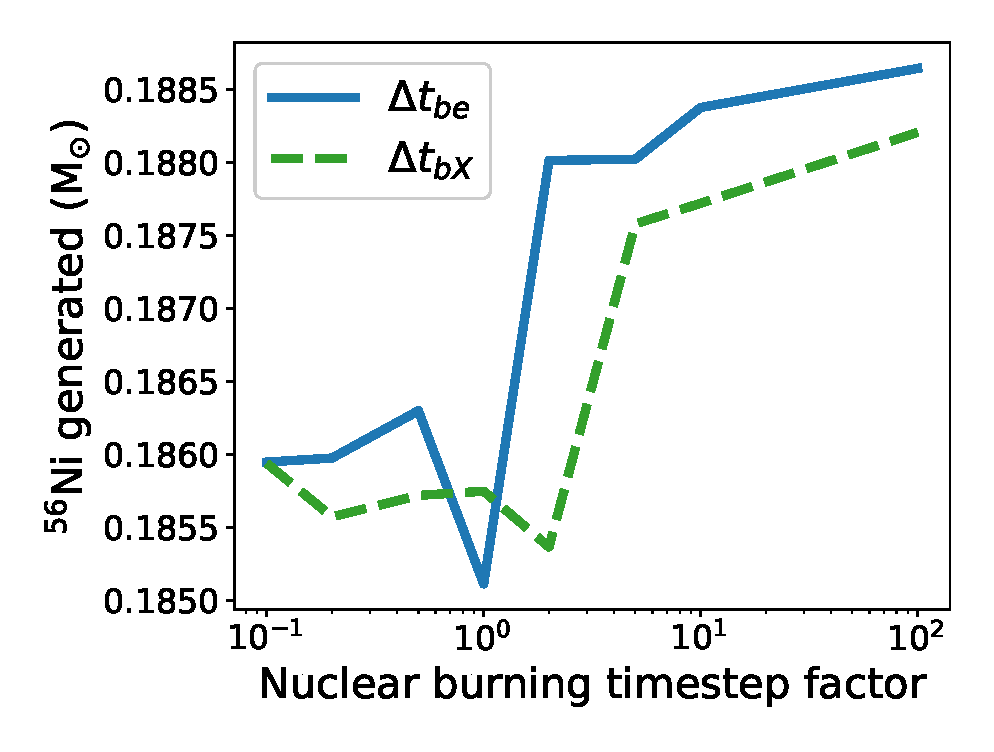
\includegraphics[scale=0.425]{{{plots/dtnuc_max_Ni56_m_P_0.64_m_S_0.64}}}
  \caption{Nickel production as a function of the timestep factors $f_{be}$
           (solid blue, limiting the timestep on changes in internal energy) and
           $f_{bX}$ (dashed green, limiting the timestep on changes in species).
           For a given $f_{be}$, $f_{bX}$ with the same value typically limits
           the timestep by at least an order of magnitude more.
           \label{fig:timestep_factor}}
\end{figure}
\autoref{fig:timestep_factor} demonstrates the effect of both parameters on the nickel
production (these limiters are somewhat redundant in the sense that a given $f_{bX}$
roughly corresponds to another (higher) $f_{be}$, as is evident by the fact that on
the graph the curves look qualitatively similar in shape but with a horizontal offset.
As either $f$ becomes small, the restriction on the timestep becomes quite severe:
for $f_{be} = 0.001$, the minimum timestep in the simulation is smaller than
$5 \times 10^{-9}\ \text{s}$ and the full simulation requires over 100,000 timesteps.
Such a simulation would be prohibitively expensive for a high resolution 3D calculation.
It is clear, though, that the timestep effect has converged when $f_{be} \sim 0.1$. We
agree that the use of values in this range by \cite{raskin:2010}, \cite{hawley:2012},
and \cite{kushnir:2013} is appropriate.

%TODO: update the above with more recent data.





%==========================================================================
% Resolution Dependence
%==========================================================================
\section{Spatial Resolution}
\label{sec:spatialresolution}



%==========================================================================
% Conclusions
%==========================================================================
\section{Conclusions and Discussion}\label{Sec:Conclusions and Discussion}
\label{sec:conclusion}



\acknowledgments

This research was supported by NSF award AST-1211563 and DOE/Office of
Nuclear Physics grant DE-FG02-87ER40317 to Stony Brook. An award of
computer time was provided by the Innovative and Novel Computational
Impact on Theory and Experiment (INCITE) program.  This research used
resources of the Oak Ridge Leadership Computing Facility located in
the Oak Ridge National Laboratory, which is supported by the Office of
Science of the Department of Energy under Contract
DE-AC05-00OR22725. Project AST106 supported use of the ORNL/Titan
resource.  This research used resources of the National Energy
Research Scientific Computing Center, which is supported by the Office
of Science of the U.S. Department of Energy under Contract
No. DE-AC02-05CH11231. The authors would like to thank Stony Brook
Research Computing and Cyberinfrastructure, and the Institute for
Advanced Computational Science at Stony Brook University for access
to the high-performance LIred and SeaWulf computing systems, the latter
of which was made possible by a \$1.4M National Science Foundation grant (\#1531492).

This research has made use of NASA's Astrophysics Data System 
Bibliographic Services. In addition, this research has made use
of the AstroBetter blog and wiki.

\software{\amrex\ (\url{https://github.com/AMReX-Codes/Amrex}),
          \castro\ \citep{castro} (\url{https://github.com/AMReX-Astro/Castro}),
          \wdmerger\ \citep{wdmergerI} (\url{https://github.com/AMReX-Astro/wdmerger}),
          GCC (\url{https://gcc.gnu.org/}),
          python (\url{https://www.python.org/}),
          matplotlib \citep{matplotlib} (\url{http://matplotlib.org/}),
          yt \citep{yt} (\url{http://yt-project.org/})}

\clearpage

\bibliographystyle{../aasjournal}
\bibliography{../refs}

\end{document}
